
\begin{frame}
  \frametitle{Cel pracy}
	{Celem pracy jest implementacja aplikacji wykonującej kompilację języka JavaScript do kodu pośredniego wykonywalnego na platformie .NET oraz porównania zaimplementowanych w języku JavaScript testowych algorytmów uruchamianych na platformie Node.js oraz .NET.}
\end{frame}

\begin{frame}
  \frametitle{Zakres pracy}
  \begin{itemize}
    \item  Opis pojęć i technologii wykorzystanych w projekcie oraz nawiązujących do tematu pracy.
    \item  Analiza języka JavaScript
    \item  Określenie zakresu implementacji
    \item  Implementacja aplikacji kompilatora
    \item  Wybór oraz implementacja algorytmów testujących
    \item  Przeprowadzenie testów i zebranie wyników
    \item  Podsumowanie wyników
  \end{itemize}
\end{frame}

\begin{frame}
  \frametitle{Wykorzystane narzędzia}
  
  \begin{block}{Implementacja kompilatora:}
    \begin{itemize}
      \item  Platforma \textit{.NET core 3.1}
      \begin{itemize}
        \item  Język C\#
      \end{itemize}
      \item ANTLR 4.8
  \end{itemize}
  \end{block}

  \begin{block}{Implementacja kodu testującego:}
    \begin{itemize}
      \item  Platforma \textit{Node.js 10.15}
      \begin{itemize}
        \item  Język JavaScript
      \end{itemize}
      \item  Platforma \textit{.NET Framework v4.0}
      \begin{itemize}
        \item  Język C\#
        \item  Język JScript
      \end{itemize}
    \end{itemize}
  \end{block}
  
\end{frame}

\begin{frame}
  \frametitle{Wykorzystane narzędzia cd.}
  
  \begin{block}{Narzędzia testujące:}
    \begin{itemize}
      \item  Dekompilacja kodu:
      \begin{itemize}
        \item  Platforma \textit{.NET Framework v4.0}
        \item  JetBrains dotPeek 2020.2.1
      \end{itemize}
      \item  Pomiar czasu i wielkości plików wykonywalnych:
      \begin{itemize}
        \item  PowerShell 7.1.1
      \end{itemize}
      \item  Pomiar zużycia pamięci:
      \begin{itemize}
        \item  JetBrains dotMemory 2020.2.1
      \end{itemize}
    \end{itemize}
  \end{block}
  
  \begin{block}{Narzędzia pomocnicze:}
    \begin{itemize}
      \item  Skrypty pomocnicze
      \begin{itemize}
        \item  PowerShell 7.1.1
      \end{itemize}
  \end{itemize}
  \end{block}
\end{frame}

\begin{frame}
  \frametitle{Konstrukcja kompilatora}
  \begin{figure}[ht]
    \centering
    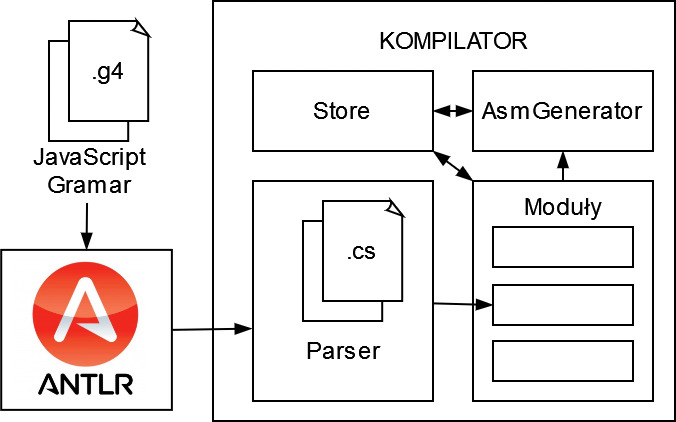
\includegraphics[width=\textwidth]{konstrukcja.jpg}
	\end{figure}
\end{frame}

\begin{frame}
  \frametitle{Sposób działania}
  \begin{figure}[ht]
    \centering
    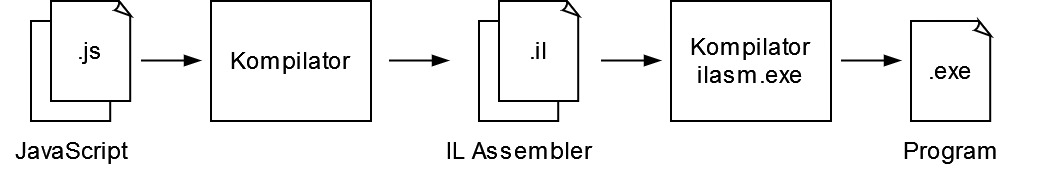
\includegraphics[width=\textwidth]{kompilacja.jpg}
	\end{figure}
\end{frame}

\begin{frame}
  \frametitle{Przygotowanie testów}
  \begin{block}{Zakres testów:}
  \begin{itemize}
    \item  Testy dla poszczególnych modułów
    \item  Implementacja oraz przygotowanie algorytmów odnalezionych w Internecie
    \begin{itemize}
      \item  Algorytm sortowania bąbelkowego
      \item  Algorytm liniowego przeszukiwania
    \end{itemize}
  \end{itemize}
  \end{block}
  \begin{block}{Przygotowanie implementacji algorytmów:}
    \begin{itemize}
      \item  Niewielka modyfikacja implementacji.
      \item  Przygotowanie odpowiedników w języku:
      \begin{itemize}
        \item JScript
        \item C\#
      \end{itemize}
    \end{itemize}
    \end{block}
\end{frame}

\begin{frame}
  \frametitle{Kryteria testów}
  \begin{block}{Testy modułów}
    \begin{itemize}
      \item  Porównanie wyniku wykonania programów
      \item  Porównanie generowanego kodu assemblera
    \end{itemize}
  \end{block}
  \begin{block}{Testy algorytmów}
    \begin{itemize}
      \item  Pomiar czasu wykonywania programów
      \item  Pomiar zużycia pamięci
      \item  Pomiar wielkości plików programów
    \end{itemize}
  \end{block}
\end{frame}

\begin{frame}
  \frametitle{Wyniki testów algorytmów}
  \begin{block}{Pomiar czasu wykonywania programów}
    
  \end{block}
\end{frame}

\begin{frame}
  \frametitle{Wyniki testów algorytmów}
  \begin{block}{Pomiar zużycia pamięci}
    
  \end{block}
\end{frame}

\begin{frame}
  \frametitle{Wyniki testów algorytmów}
  \begin{block}{Pomiar wielkości plików programów}
    
  \end{block}
\end{frame}

\begin{frame}
  \frametitle{Podsumowanie}
  \begin{itemize}
    \item  Przy analizie wyników poszczególnych testów funkcjonalności zostały wykazane niewielkie różnice przy wyświetlaniu elementów na
    konsoli.
    \item Porównanie generowanego kodu assemblera wykazało słabą optymalizacją stworzonego kompilatora.
    \item Testów algorytmów pokazują porównywalne wyniki dla kodu kompilowanego z języka C\# oraz lepsze wyniki w porównaniu do kodu JScript.
  \end{itemize}
\end{frame}

\begin{frame}
  \frametitle{Kierunki dalszych prac}
  \begin{block}{Przykłady:}
    \begin{itemize}
      \item  Implementacja pełnej funkcjonalności języka JavaScript
      \item  Zastosowanie pełnej gamy instrukcji asemblerowych
      \item  Testy na bardziej złożonych algorytmach lub bibliotekach
      \item  Optymalizacja generowanego kodu assemblera
      \item  Dodanie mechanizmów zrównoleglania kodu
    \end{itemize}
  \end{block}
\end{frame}

\begin{frame}
	\begin{center}
	\Huge Dziękuję za uwagę
	\end{center}
\end{frame}
